Chapter 4's results suggest that methods addressing model dependence on positional cues can be an effective way to boost summarization performance. The previous chapter's auxiliary loss method is able to decrease how frequently the base model selects from leading sentences, while also significantly improving summary quality. Although the auxiliary loss method's summarization improvement is statistically significant, it does not offer extraordinary gains over baselines. Figure \ref{fig:avg_pos} reveals that the method only offers modest reductions in how often lead sentences are selected and does not approach the percentage an oracle summarizer selects from the lead.

The results do not necessarily suggest that addressing positional biases is an ineffective strategy. Previous works such as \cite{kedzie2018content} and our own experiments in Chapter 3 have already shown that positional cues represent a major bottleneck for learning summarization. Instead, we suspect that the auxiliary loss methods are not sufficiently aggressive enough to counter the effects of lead bias. For these reasons, we would prefer a model formulation that integrates the ideas of lead bias more centrally.

We hypothesize that articles with a strong lead (i.e. the lead forms an accurate summary) are fundamentally different from cases with a weak lead, such that a classifier could distinguish between these two cases. We look to build such a classifier, so that we can apply different summarization strategies for the two scenarios. In this chapter, we detail this new classification task, the model formulation, the challenges surrounding the task and the resulting model's summarization capabilities.

\section{Classification Task}
We first define how to categorize articles based on the lead baseline's strength. Since there is a large variance between the highest achievable ROUGE score between different articles, we avoid categorizing articles solely based on the lead ROUGE score. For example, if the lead baseline achieves 30.0 ROUGE-1 on both articles $A$ and $B$, but the oracle summarizer respectively achieves 60.0 and 30.0 ROUGE-1, we should avoid placing $A$ and $B$ in the same category. To avoid this scenario, we rank articles by how well the lead performs in relation to an oracle summarizer:

\begin{equation}
\mathrm{Proportion\ Score}(D) = \frac{r_{lead}(D)}{r_{oracle}(D)}
\end{equation}
where $r_{lead}$ denotes the lead-3's ROUGE-1, -2 and -L average score on $D$, and $r_{oracle}$ denotes the same quantity using an oracle summarizer.
As previously, the lead is defined as the first 3 sentences in the document, while the oracle is defined in the same way as in Chapter \ref{chap:aux_loss}.

We also need to define a threshold value $T$ in order to divide articles. To determine an acceptable threshold value, we experiment with varying threshold values on the CNN / Daily Mail development set. For each threshold value, we divide the articles based on whether their proportion score falls below or above the given threshold. Documents below the threshold are summarized by the BandiSum+KL model, while documents above the threshold are handled by the lead-3 baseline. The results are shown in Figure \ref{fig:prop_value_thresh}.

\begin{figure}[h]
    \centering
    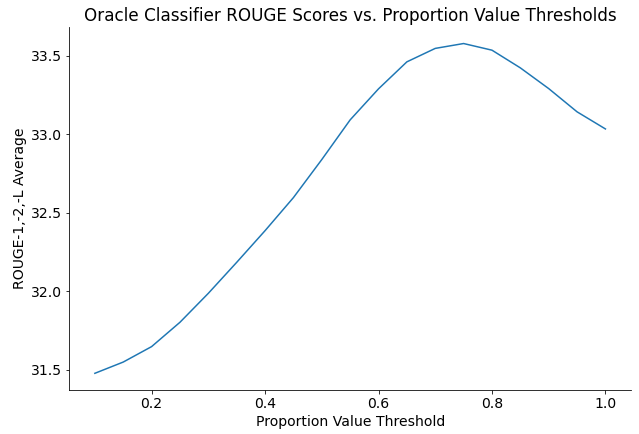
\includegraphics[width=0.75\linewidth]{fig/proportion_value_thresholds.png}
    \caption[ROUGE performance with varying proportion score thresholds.]{Each data point in this figure represents a trial with varying threshold $T$. In each trial, articles with proportion scores $<T$ are summarized by BanditSum+KL and otherwise summarized by the lead-3 baseline. The highest $\frac{1}{3}(R1+R2+RL)$ value is attained when $T = 0.75$.}
    \label{fig:prop_value_thresh}
\end{figure}

The highest gains in ROUGE performance are attained when the threshold $T = 0.75$, and we therefore use this value as the threshold in the following experiments.

Since distinguishing points very close to the threshold may be difficult for classifiers, we also experiment with removing articles close to the threshold $T$. After ranking all articles by their proportion score, we create subsets by removing articles close to the threshold. Specifically, we experiment with removing 20, 30, 50 and 60 percent from each of the training / development / testing data, centered around $T$. The subsets are named \Dtwenty, \Dthirty, \Dfifty{} and \Dsixty. We use \Dall{} to refer to the full dataset with no data removed. Furthermore, we designate the subset of articles with a proportion score less than $T$ as \Dlate, and greater than $T$ as \Dearly.

\section{Models}
In this section, we introduce the various components that comprise our summarization model. We describe (1) a strong baseline using BanditSum and BERT, (2) the neural classifier model, and (3) the \BanSumEarly{} and \BanSumLate{} models for the \Dearly{} and \Dlate{} subsets.

\subsection{Neural Classifier}
The centrepiece of our summarization approach is a classifier separating articles with a strong lead from articles where summary-worthy sentences appear later. We experiment with four model formulations. A common element of these models is they encode the leading three sentences separately from the overall document and recombine the embeddings to classify the article. The goal of this formulation is to allow the model to learn the interactions between the article's leading sentences and the overall document, in order to properly classify the article. The four models are as follows:
\begin{itemize}
    \item \textbf{Concatenation model:} After separately encoding the first three leading sentences and the entire document with BERT, we extract the [CLS] token embeddings as sentence representations. We then use separate LSTMs to run over the lead and document sentence embeddings, extracting the final hidden state of both. Shallow MLPs encode these representations to form a \textit{lead representation} $\mathbf{h}_L$ and a \textit{document representation} $\mathbf{h}_D$. Finally the lead and whole document representations are concatenated and a logistic layer assigns a probability of a high proportion score:
    \begin{equation}
        p\left(\frac{r_{lead}(D)}{r_{oracle}(D)} > T \ \middle\vert\  \mathbf{h}_L, \mathbf{h}_D \right) = \sigma \left(w_{out}\ [ \mathbf{h}_L ; \mathbf{h}_D ] \right)
    \end{equation}
    
    \item \textbf{Bilinear model:} This model is similar to the concatenation model but instead of concatenating the lead and document representations, a bilinear map combines the embeddings.
    \begin{equation}
        p\left(\frac{r_{lead}(D)}{r_{oracle}(D)} > T \ \middle\vert\  \mathbf{h}_L, \mathbf{h}_D \right) = \sigma \left( \mathbf{h}_L^T W_{out}\ \mathbf{h}_D \right)
    \end{equation}
    
    \item \textbf{Separate-BERT model:} This model follows the concatenation model but separate BERT encoders are used to produce the lead and document representations.
    \item \textbf{No-lead baseline:} The leading three sentences are not separately encoded. After BERT encodes the document, the first [CLS] token representation is provided as input to a logistic layer which maps this output to a probability between 0 and 1.
\end{itemize}

\subsection{\Dearly{} and \Dlate{} Subset Training}
After articles are classified, our approach requires two different summarization methods to handle each case. A reasonable strategy is to train separate summarization systems on the \Dearly{} and \Dlate{} subsets. We first define a base model based on BanditSum, then detail how to specialize the model on the two cases through subset training.

\subsubsection{Base Model: BanditSum+BERT}
% Describe the new model architecture and the table below
We continue to use BanditSum in these experiments, though we replace the sentence encoder from the original formulation with BERT \parencite{bert}. Given a document $D$ with sentences $s_1,\dots,s_N$, we encode it using BERT and use the [CLS] token as a sentence embedding, similar to the BertSum summarization model \parencite{bertsum}. These sentence embeddings are then fed to a multi-layer perceptron decoder in order to produce a \textit{sentence affinity} $\pi_i \in [0, 1]$ for each sentence $s_i \in D$. Essentially, we compute:

\begin{align}
    \pi_i &= \mathrm{MLP}(h_i) \\
    h_1,\dots,h_N &= \mathrm{BERT}(D)
\end{align}

The MLP structure follows BanditSum's decoder specifications and the remaining model details such as the reinforcement learning-based objective function follow BanditSum's details as well \parencite{dong2018banditsum}.

\subsubsection{Training on Data Subsets}
In order to specialize the base model towards summarizing \Dearly{} and \Dlate{} articles, we train two separate versions of BanditSum+BERT, restricted to the \Dearly{} and \Dlate{} subsets. Our hypothesis is that articles where the lead baseline performs well require a different summarization strategy than cases where the lead is weak. We use \BanSumEarly{} to denote the model trained on \Dearly{} and likewise, use \BanSumLate{} for the model trained on \Dlate{}.

\subsection{Summarization through Classification: LeadClassifySum}
The final summarization model is a straightforward pipeline of the previous components. Given an article, the classifier predicts if it belongs in \Dearly{} or \Dlate{}, and the appropriate model is then used to summarize it. After finding that \BanSumEarly{} solely learns positional cues and chooses indices nearly always matching the lead-3 baseline, we instead use the simpler lead-3 baseline to summarize cases in \Dearly{}. We use \BanSumLate{} to summarize articles in \Dlate{}. This final model is named LeadClassifySum.

\section{Experiments}
% Classifier
For each of the \Dtwenty{}, \Dthirty{}, \Dfifty{} and \Dsixty{} subsets, we train the four classification models to separate articles with a proportion score less than $T$ from ones greater than $T$. We also experiment with a setting where no articles are removed, i.e. using \Dall{}. Every model is trained to reduce the cross-entropy loss between its prediction and the gold label. For each training subset, we test the model using a subset of the test set that respects the same threshold boundaries as the training subset. We implement data re-weighting to reduce the effects of class imbalance, and we employ gradient clipping with a maximum gradient norm of 1.0.

% Base model
We train the BanditSum+BERT model on the CNN / Daily Mail dataset, converging after 6 epochs. For both \Dearly{} and \Dlate{} subsets, we train separate BanditSum+BERT models, with the late version converging within 10 epochs and the early version within 5 epochs.

For all experiments, we employ the Hugging Face `bert-base-uncased' BERT implementation to build our models \parencite{Wolf2019HuggingFacesTS}. We use Adam to optimize model parameters, with PyTorch's default momentum configuration \parencite{adam_kingma2014adam, pytorch}. We tune the learning rate for each of these experiments using the Tune library \parencite{tune}.

\section{Results}
\subsection{Classification Results}
Results across all model variations are very similar for at least one learning rate configuration. The results for the Bilinear model are shown in Table \ref{tab:class_acc}. All subsets experience a striking degree of overfitting, with each subset resulting in greater than 20\% difference between the training and testing accuracy. In Table \ref{tab:maj_base_comp}, we compare the Bilinear model to a simple majority baseline. Apart from the \Dall{} setting, the classifier outperforms the majority baseline, suggesting that the classifier learns non-trivial cues from the training data. There is also a notable increase in test set accuracy as the amount of data removed increases, with an 11\% increase between the \Dall{} and \Dsixty{} dataset. However, overall, overfitting prevents our classifier implementations from being practical.

\begin{table}[h]
    \centering
    \begin{tabular}{c|c|c}
    \toprule
    Dataset	&	Training Accuracy (\%)	&	Test Accuracy (\%)	\\ \hline
    \Dall	&	81.64	&	62.5	\\
    \Dtwenty	&	90.29	&	65.09	\\
    \Dthirty	&	95.74	&	67.09	\\
    \Dfifty	&	93.31	&	71.9	\\
    \Dsixty	&	93.61	&	73.49	\\ \bottomrule
    \end{tabular}
    \caption[Classification results for the Bilinear model on various data subsets.]{Classification results for the Bilinear model on various data subsets. We notice greater test accuracy as the amount of data removed increases; however, strong overfitting prevents the classifiers from being practical for our purposes.}
    \label{tab:class_acc}
\end{table}

\begin{table}[h]
    \centering
    \begin{tabular}{c|c|c|c|c|c}
    \toprule
    Model	&	\multicolumn{5}{c}{Accuracy (\%)}		\\	
    &	\Dall{}	&	\Dtwenty{}	&	\Dthirty{}	&	\Dfifty{}	&	\Dsixty{}	\\ \hline
    Majority Baseline	&	64.62	&	52.61	&	52.94	&	53.29	&	53.16	\\
    Bilinear Model	&	62.5	&	65.09	&	67.09	&	71.9	&	73.49	\\ \bottomrule
    \end{tabular}
    \caption[Classification accuracy comparison for the bilinear model against a majority baseline.]{Apart from the \Dall{} dataset, the Bilinear model is able to outperform a majority baseline on the classification task.}
    \label{tab:maj_base_comp}
\end{table}

\subsection{\Dearly{} and \Dlate{} Results}
% D_late results
The results for \Dlate{} and \Dearly{} are displayed in Tables \ref{tab:late_subset} and \ref{tab:early_subset} respectively. On \Dlate{}, subset training benefits the BanditSum+BERT model considerably, as we see large jumps in ROUGE-1, -2 and -L metrics. There is also a strong decrease in the lead overlap, as the \BanSumLate{} model is exposed to less positional bias compared to the baseline model. These results confirm that separating articles with weak lead performance is important for summarization, and that subset training can help models focus on a specific strategy for the \Dlate{} subset.

% D_early results
The \Dearly{} experiment shows even greater gains in ROUGE performance, around 2 points across all three ROUGE metrics. However, in this case, positional biases clearly play a dominating role in the model's learning process, as the model exactly copies the lead-3 baseline and achieves the same performance. Unfortunately, the model fails to pick up on deeper cues and its ROUGE scores remain far from the oracle's.

\begin{table}[t]
    \centering
    \begin{tabular}{c|c|c|c|c}
    \toprule
    Model	&	ROUGE-1	&	ROUGE-2	&	ROUGE-L	&	Lead Overlap (\%)	\\ \hline
    BanditSum+BERT	&	40.17	&	17.56	&	36.61	&	53.20	\\ 
    \BanSumLate	&	40.75	&	18.17	&	37.30	&	33.37	\\ \hline
    Lead-3	&	35.32	&	13.38	&	31.77	&	100.0	\\ 
    Oracle	&	57.19	&	33.50	&	53.94	&	17.13	\\
    \bottomrule
    \end{tabular}
    \caption[ROUGE results on \Dlate{}.]{Results on CNN / Daily Mail test articles with proportion score less than $T = 0.75$, corresponding to training on \Dlate. The \BanSumLate{} model noticeably outperforms BanditSum+BERT and selects the leading sentences less often.}
    \label{tab:late_subset}
\end{table}

\begin{table}[t]
    \centering
    \begin{tabular}{c|c|c|c|c}
    \toprule
    Model &	ROUGE-1	&	ROUGE-2	&	ROUGE-L	&	Lead Overlap (\%)	\\ \hline
    BanditSum+BERT	&	47.01	&	22.84	&	43.18	&	67.50	\\
    \BanSumEarly	&	49.01	&	24.52	&	45.04	&	99.99	\\ \hline
    Lead-3	&	49.01	&	24.52	&	45.04	&	100.0	\\
    Oracle	&	56.16	&	30.70	&	52.45	&	45.70	\\ \bottomrule
    \end{tabular}
    \caption[ROUGE results on \Dearly{}.]{Results on CNN / Daily Mail test articles with proportion score less than $T = 0.75$, corresponding to training on \Dearly. Although \BanSumEarly{} outperforms BanditSum+BERT significantly, positional cues dominate the learning signal for \BanSumEarly{}. In the end, it is indistinguishable from the lead-3 baseline.}
    \label{tab:early_subset}
\end{table}

\subsection{Summarization Results}
The main summarization results on the CNN / Daily Mail test set are shown in Table \ref{tab:banditsum_bert}. 

\subsubsection{BanditSum+BERT Baseline}
The BanditSum+BERT markedly outperforms BanditSum across all three ROUGE metrics, indicating that BERT's encodings are far more suitable for this summarization task than LSTMs. Besides a noticeable increase in ROUGE, the model also selects significantly less from the lead than both BanditSum and the BanditSum+KL model. One possible explanation is that BERT acts as a regularizer for sentence position, and its strong language modelling abilities help it from being distracted by position cues.

\subsubsection{LeadClassifySum}
Hampered by a weak classifier, the LeadClassifySum approach is unable to surpass its baseline in terms of ROUGE. Curiously, the degree of lead overlap actually increases, further reflecting on the classifier's inability to properly separate strong-lead articles from weak ones. The summarization approach hinges on a capable classifier, and in the absence of one, this result is expected.

\begin{table}[h]
    \centering
    \begin{tabular}{c|c|c|c|c}
    \toprule
    Model	&	ROUGE-1	&	ROUGE-2	&	ROUGE-L	&	Lead Overlap (\%)	\\ \hline
    Lead-3	&	40.06	&	17.53	&	36.18	&	100.0	\\
    BanditSum 	&	41.68	&	18.78	&	38.00	&	69.87	\\
    BanditSum+BERT	&	42.70	&	19.40	&	39.03	&	57.52	\\ \hline
    LeadClassifySum	&	41.82	&	18.62	&	38.12	&	73.52	\\ \hline
    Oracle Classifier	&	43.73	&	20.49	&	40.13	&	52.02	\\
    Oracle	&	56.53	&	32.65	&	53.12	&	27.24	\\ \bottomrule
    \end{tabular}
    \caption[LeadClassifySum ROUGE results on CNN / Daily Mail test set.]{Results from various models on the CNN / Daily Mail test set. While BanditSum+BERT outperforms BanditSum, both are surpassed by the Oracle Classifier and true Oracle scores.}
    \label{tab:banditsum_bert}
\end{table}

\section{Analysis}
\subsection{Exploring Threshold Values}
\begin{figure}[h]
    \centering
    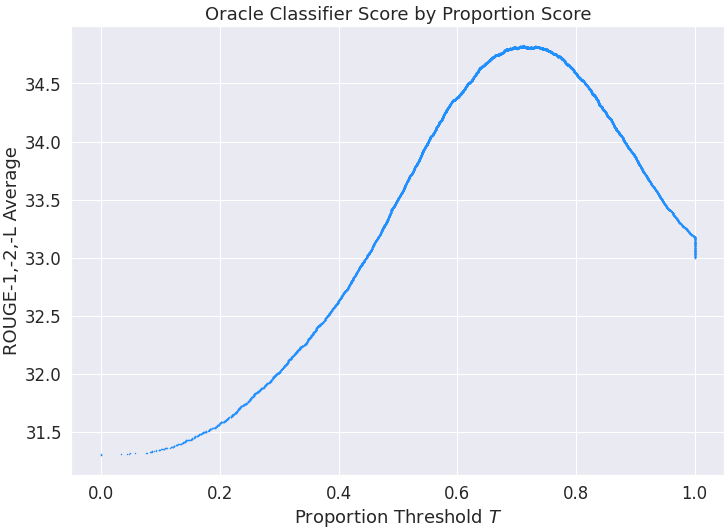
\includegraphics[width=0.75\linewidth]{fig/oracle_lead_classifier_thresholds.png}
    \caption[A fine-grained analysis of summarization performance change when the threshold is varied.]{By running both \BanSumLate{} and Lead-3 models over the entire test set, we can visualize how the ROUGE-1, -2 and -L average score changes on an article-by-article basis when varying the threshold $T$. This experiment validates our choice of $T$ and shows that only a single optimum exists.}
    \label{fig:oracle_classifier_threshold}
\end{figure}

A natural question to ask is what an upper performance bound would be from using this approach. To this end, we run an oracle classifier over the CNN / Daily Mail test set to correctly label articles with their proportion score. Articles with a proportion score less than $T$ are then summarized with the \BanSumLate{} model. Conversely, articles with a proportion score greater than $T$ are summarized by the lead-3 baseline.

The Oracle Classifier results are displayed in Table \ref{tab:banditsum_bert}. The noticeable performance gain of over 1 point in ROUGE-1, -2 and -L metrics suggest that our lead classifier approach is a viable approach to summarization. This oracle method is furthermore able to decrease lead overlap by 5.5\% compared to the base \BanSumLate{} model, achieving a closer degree of lead overlap as the true oracle model.

We also want to further validate our choice of $T$. The experiment shown in Fig. \ref{fig:prop_value_thresh} gives an adequate estimate of a good threshold value. However, we would prefer to use stronger baselines as the base models and analyze the results on a fine-grained article-by-article basis.

We first create summaries for the whole CNN / Daily Mail test set with both lead-3 and \BanSumLate{} models, and sort all articles by their proportion scores. We then sweep through the sorted test set, marking the change in overall average ROUGE-1, -2 and -L scores as $T$ varies. The results are shown in Figure \ref{fig:oracle_classifier_threshold}. The peak ROUGE score, occurring at $T=0.71$, shows the possible gains over the \BanSumLate{} model (far right point) and lead-3 model (far left point). Figure \ref{fig:oracle_classifier_threshold} also demonstrates that only a single optimal threshold value exists, and that our choice of $T$ is justified.

\subsection{Classifier Regularization}
In an effort to reduce the degree of overfitting, we explore a variety of regularization techniques to reduce the gap between the training and testing accuracies. We experiment with the following techniques:
\begin{itemize}
    \item \textbf{Weight decay} is a common technique for regularizing parameters which involves multiplying each weight by a factor slightly less than one after each step. We explore a variety of weight decay terms to regularize model parameters.
    \item \textbf{Reducing model complexity:} We halve both the LSTM decoders' hidden size and the logistic classifier size to explore if reducing model size improves generalization.
    \item \textbf{PCA on BERT outputs:} BERT's output representations are 768-dimensional vectors, which may be too large for the task. Using a version of BERT with lower-dimensional outputs requires re-training the entire BERT model from scratch, which is computationally infeasible. Instead, after fine-tuning BERT on the classification task, we fix BERT's parameters and employ PCA to reduce the output dimension to 300. We then continue fine-tuning the decoders using the lower-dimensional outputs.
    \item \textbf{Freeze BERT outputs:} In order to reduce the number of trainable parameters, we fix BERT's parameters, and only fine-tune the remaining weights.
\end{itemize}
We do not explore using dropout as the BERT encoder already employs it.

Unfortunately, none of the above regularization techniques significantly changes classification accuracy on the test set. Freezing BERT outputs decreases accuracy by around 8\%. Further regularization techniques may be beneficial to the task, but ultimately the solution may require alternate model formulations to overcome the gaps in accuracy.

\vspace{-4px}
\section{Conclusion}
In this chapter, we conjecture that separating articles with strong or weak leads can aid automatic summarization. To partition the dataset, we define a document's \textit{Proportion Score}, the ratio of the lead to oracle ROUGE score. We run experiments using the lead-3 baseline and the BanditSum+KL model to determine an effective threshold $T$ to partition the CNN / Daily Mail dataset.

We design classifiers to divide documents by their proportion score. Despite regularization attempts, overfitting remains a bottleneck for our approach. Future methods may require alternate model formulations or stronger regularization techniques.

We proceed to build a base model using BanditSum with a BERT encoder, and show that this model outperforms the original BanditSum summarizer. After partitioning the training dataset based on proportion score, we train separate summarizers on the subsets. On the late subset, where the documents' proportion scores are less than $T$, \BanSumLate{} is able to create better summaries, presumably because its representations are less biased towards positional cues. In contrast, \BanSumEarly{} summarization performance increases on the early subset, but the model exclusively learns to copy the lead baseline.

Using an oracle classifier, we show that the summarization performance can improve up to 1 point across all ROUGE-1, -2 and -L metrics. We examine how performance gains change on an article-by-article basis, showing that only a single optimum occurs at $T = 0.71$.
